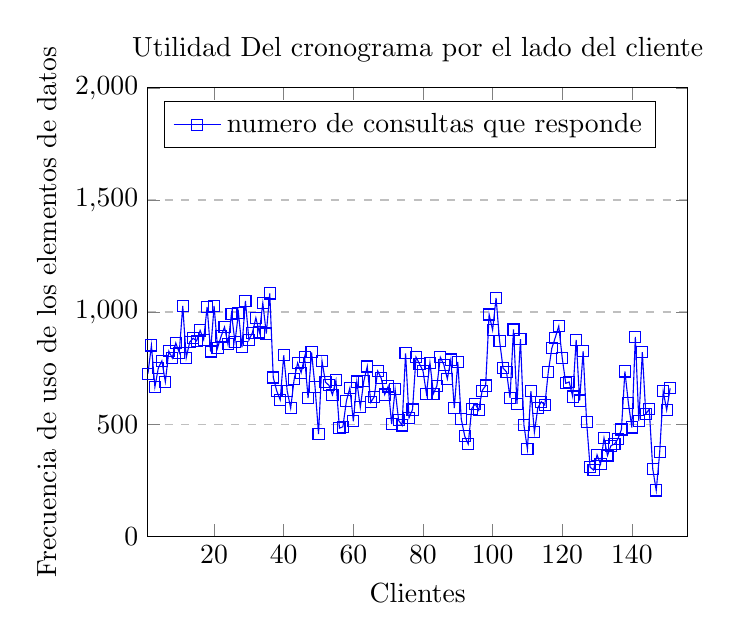
\begin{tikzpicture}
\begin{axis}[
    title={Utilidad Del cronograma por el lado del cliente},
    xlabel={Clientes},
    ylabel={Frecuencia de uso de los elementos de datos},
    xmin=1, xmax=156,
    ymin=0, ymax=2000,
    xtick={},
    ytick={},
    legend pos=north west,
    ymajorgrids=true,
    grid style=dashed,
]

\addplot[
    color=blue,
    mark=square,
    ]
    coordinates {
    %USO EXACTO
    (1,725)
(2,851)
(3,666)
(4,751)
(5,782)
(6,689)
(7,825)
(8,795)
(9,862)
(10,819)
(11,1027)
(12,796)
(13,866)
(14,883)
(15,871)
(16,918)
(17,877)
(18,1023)
(19,824)
(20,1027)
(21,840)
(22,891)
(23,933)
(24,856)
(25,993)
(26,866)
(27,996)
(28,843)
(29,1050)
(30,875)
(31,907)
(32,974)
(33,909)
(34,1040)
(35,904)
(36,1083)
(37,708)
(38,648)
(39,608)
(40,807)
(41,648)
(42,571)
(43,700)
(44,773)
(45,729)
(46,799)
(47,616)
(48,820)
(49,666)
(50,456)
(51,781)
(52,687)
(53,673)
(54,631)
(55,695)
(56,482)
(57,488)
(58,603)
(59,661)
(60,513)
(61,690)
(62,575)
(63,691)
(64,757)
(65,597)
(66,622)
(67,737)
(68,705)
(69,632)
(70,668)
(71,500)
(72,655)
(73,517)
(74,494)
(75,816)
(76,528)
(77,565)
(78,799)
(79,769)
(80,738)
(81,636)
(82,774)
(83,636)
(84,671)
(85,798)
(86,765)
(87,702)
(88,788)
(89,571)
(90,777)
(91,522)
(92,446)
(93,411)
(94,569)
(95,590)
(96,562)
(97,649)
(98,672)
(99,989)
(100,920)
(101,1063)
(102,872)
(103,750)
(104,733)
(105,617)
(106,922)
(107,590)
(108,879)
(109,495)
(110,388)
(111,647)
(112,464)
(113,573)
(114,600)
(115,585)
(116,734)
(117,838)
(118,886)
(119,937)
(120,795)
(121,682)
(122,688)
(123,623)
(124,876)
(125,605)
(126,825)
(127,510)
(128,308)
(129,295)
(130,363)
(131,321)
(132,438)
(133,360)
(134,404)
(135,411)
(136,434)
(137,476)
(138,735)
(139,594)
(140,485)
(141,889)
(142,514)
(143,821)
(144,546)
(145,566)
(146,300)
(147,204)
(148,376)
(149,646)
(150,563)
(151,660)
    };
    \legend{numero de consultas que responde}

\end{axis}
\end{tikzpicture}

